\documentclass[preprint,12pt]{elsarticle}
\usepackage{amsmath,amssymb,bm,booktabs,graphicx,hyperref}
\usepackage[margin=25mm]{geometry}
\graphicspath{{figures/}}
\journal{LBFlow research manuscript}
\makeatletter
\def\ps@pprintTitle{%
  \let\@oddhead\@empty\let\@evenhead\@empty
  \def\@oddfoot{\footnotesize\itshape Research draft\hfill\today}%
  \let\@evenfoot\@oddfoot}
\makeatother
\emergencystretch=3em
\newcommand{\vct}[1]{\bm{#1}}
\begin{document}
\begin{frontmatter}
\title{LBFlow: reproducible verification of an MPI color-gradient lattice Boltzmann solver}
\author{Yu Zhou\corref{cor1}}
\address{Independent Researcher}
\ead{[private contact omitted]}
\cortext[cor1]{Corresponding author.}
\begin{abstract}
LBFlow, is a C++ lattice Boltzmann
solver for single-component and immiscible
two-component flow on D2Q9 and D3Q19 lattices. Its voxel input, geometrical
wetting treatment and MPI decomposition support a compact workflow for
numerical experiments. We reconstruct the implemented operators and develop
a reproducible verification package around the historical solver. Decisive
counterexamples identify incorrect second-phase MRT relaxation, an
incompatible shifted-equilibrium force treatment, and premature termination
based on saturation. Local moment relaxation, consistent forcing, explicit
restart timing and field-based stopping restore the expected behavior.
Uniform acceleration agrees with its analytic reference to roundoff;
halfway-wall MRT channel profiles agree to approximately $10^{-8}$ relative
error at the tested stopping times. Laplace tests quantify finite-interface
pressure errors in two and three dimensions. Layered flow distinguishes
interpolation bias from collision error. A wall-stencil ablation finds that
renormalization improves several contact-angle measurements but can increase
spurious velocity. The contribution is the inspectable implementation and
verification evidence, rather than a new class of multiphase model.
\end{abstract}
\begin{keyword}
lattice Boltzmann \sep color gradient \sep verification \sep MPI \sep wetting \sep reproducibility
\end{keyword}
\end{frontmatter}

\noindent\textbf{Draft status.} Numerical results are generated from recorded
executions. The sole author is Yu Zhou, Independent Researcher. Source code
is licensed under MIT and has been prepared for release in the LBFlow
repository. Public availability and an immutable release citation must be
verified before submission.

\section{Motivation and significance}
Long-lived numerical software can continue producing finite fields after
changes in physical configuration expose an implementation defect. In
multiphase lattice Boltzmann calculations, conservation alone does not verify
force integration, viscosity, surface tension or wetting. DRLab provides a
useful case in which these contracts can be inspected separately.

The historical implementation combines color-gradient perturbation and
recoloring with geometrical wall treatment. These mechanisms belong to the
established color-gradient family \cite{reis2007,latva2005,liu2012,liuerratum2012}.
Direct and modified-gradient contact-angle treatments already appear in
two- and three-dimensional work \cite{leclaire2016,leclaire2017,xu2017,akai2018}.
Later comparisons and curved-wall developments continue to examine
wetting accuracy \cite{sedahmed2024,bhattacharya2026}. Our software contribution
is therefore a recoverable, tested realization of established methods, with
explicit evidence about its reliable operating range and remaining errors.

The source baseline is the reference solver, historical revision
\texttt{1bef9bbe7047}. The full source identity is recorded in the supplement. The original archive is
preserved; repairs, inputs, run receipts and analysis are maintained in a
maintained LBFlow implementation. Dates in commit messages establish source
history but are not treated as evidence of scientific priority.

\section{Software description}
\subsection{Architecture and workflow}
The code separates lattice/grid geometry, MPI exchange, parameter and field
I/O, and fluid collision operators. A byte-valued voxel file assigns initial
phases and solid or boundary labels. A parameter file selects the lattice,
relaxation operator, relaxation times, forcing and wetting. D2Q9 and D3Q19,
SRT and raw-moment MRT, and the single-component and color-fluid executables
are exercised here. The Shan--Chen placeholder is rejected explicitly.

Directional populations reside in arrays; streaming exchanges the required
neighbor data between MPI subdomains. Macroscopic fields are written as VTI
pieces that the analysis reconstructs into a complete global lattice.
Restart files contain outgoing populations and a sidecar recording the time,
lattice, phase count and next streaming action. Historical checkpoints
without an identifiable stage are rejected. A fresh convergence history is
required after restart. Exceptions and invalid populations cause a nonzero
MPI failure status.

The reproducibility scripts generate every geometry, record inputs and
executable hashes, preserve raw output and calculate independent reference
solutions. Each study uses a frozen executable so a later build cannot alter
an ongoing batch. Algebraic checks are available through CTest.

\subsection{Recovered and corrected operators}
In lattice units, the component densities and color field are
\begin{equation}
 \rho_k=\sum_i f_i^k,\quad \rho=\rho_0+\rho_1,\quad
 \chi=(\rho_0-\rho_1)/\rho,\quad
 \rho\vct u=\sum_i\vct e_i(f_i^0+f_i^1)+\vct F/2.
\end{equation}
Here $\vct F$ is force per unit volume. The mixture equilibrium is
\begin{equation}
 f_i^{eq}=\rho_0\phi_i^0+\rho_1\phi_i^1+
 \rho w_i[3\vct e_i\!\cdot\!\vct u+
 4.5(\vct e_i\!\cdot\!\vct u)^2-1.5|\vct u|^2].
\end{equation}
The phase weights give $c_{p,k}^2=3(1-\alpha_k)/5$ in D2Q9 and
$(1-\alpha_k)/2$ in D3Q19. The present quantitative tests use equal reference
densities and the standard pressure weights, so $p=\rho/3$.

The legacy arithmetic rule interpolates $\tau$ by component density fraction.
For $\varphi=\rho_0/\rho$ and $\nu_k=(\tau_k-1/2)/3$, the optional harmonic
kinematic-viscosity rule is
\begin{equation}
 \nu^{-1}=\varphi/\nu_0+(1-\varphi)/\nu_1,\qquad \tau=1/2+3\nu.
\end{equation}
The two rules are compared at equal density; equivalence to a dynamic-viscosity
law is not assumed at unequal density.

With $\vct m=M\vct f$, collision and body-force insertion become
\begin{equation}
 \vct m^*=\vct m-S(\vct m-\vct m^{eq})+(I-S/2)M\vct G,
 \quad G_i=w_i[3(\vct e_i-\vct u)+9(\vct e_i\!\cdot\!\vct u)\vct e_i]\!\cdot\!\vct F.
\end{equation}
This uses established discrete forcing and moment relaxation
\cite{guo2002,lallemand2000}. Conserved rates are zero. The retained
nonconserved rates are $s_u=1/\tau$ and $s_q=8(2-s_u)/(8-s_u)$, with
$(1/s_u-1/2)(1/s_q-1/2)=3/16$ \cite{ginzburg2003}.

Interfacial perturbation and recoloring retain the recovered structure:
\begin{align}
 \Delta_i&=\frac{9\sigma |\vct g|}{4\tau}
 \left[w_i(\vct e_i\!\cdot\!\vct n)^2-B_i\right],\quad
 \vct n=\vct g/|\vct g|,\\
 f_i^{0,*}&=\frac{\rho_0}{\rho}f_i^{post}+
 \beta\frac{\rho_0\rho_1}{\rho^2}\cos\varphi_i f_i^{eq}(\vct u=0),\qquad
 f_i^{1,*}=f_i^{post}-f_i^{0,*}.
\end{align}
The actual arrays satisfy zero perturbation mass and momentum and
$\sum_i\vct e_i\vct e_i\Delta_i=\sigma|\vct g|(\vct n\vct n-I)/(2\tau)$.
Every nonzero capillary moment is coupled to a mode with rate $s_u$.

Initialization constructs incoming rest populations with $-\vct G/2$ and
applies the normal collision kernel once. The stored state is then outgoing
at time zero. After streaming, a uniform forced domain has physical velocity
$\vct u(t)=t\vct F/\rho$. The same state convention is used for routine and
convergence-triggered checkpoints.

\subsection{Wetting and termination}
At a wall-adjacent fluid node, the historical gradient skips solid neighbors.
Writing $\mathcal F$ for the remaining stencil,
\begin{equation}
 \vct b=\sum_{i\in\mathcal F}w_i\vct e_i(\chi_i-\chi),\quad
 A=\sum_{i\in\mathcal F}w_i\vct e_i\vct e_i,
 \quad\vct g_{legacy}=3\vct b,\quad\vct g_{ren}=A^{-1}\vct b.
\end{equation}
The second expression is a standard weighted linear reconstruction, not a
new wetting model. It agrees with the bulk stencil and exactly reproduces
linear fields when $A$ has full rank. Unsupported rank-deficient stencils
are rejected. Both variants apply the same recovered angle rotation and
wall normal. On a flat lower wall, the legacy stencil scales the tangential
and normal derivatives by $5/6$ and $1/2$ respectively.

Steady termination requires finite state, stable requested scalar diagnostics,
velocity convergence and, for color flow, convergence of the spatial color
field, for three successive reports. Constant saturation cannot terminate a
translating phase field. Periodic acceleration benchmarks disable steady
stopping; undefined pressure-based permeability is identified separately
from invalid numerical state.

\section{Illustrative verification}
All runs use double precision, GCC 13.3, CMake 3.28.3 and Open MPI 4.1.6 on
Linux. Parallel execution timings are not presented as scaling results.
The tested physical range is low-speed flow at equal reference density,
$\tau_k\in\{0.6,0.8,1,1.4\}$ and prescribed $\sigma=0.005$ for droplet cases.
The supplement supplies derivations, measurement protocols and run identities.

\subsection{Force, viscosity and restart}
In the original MRT operator, $S$ was fixed at the first-phase relaxation
time. Pure second-phase pressure-channel fields were therefore identical
when its relaxation time changed. The original velocity-shift force has
momentum increment $s_j\tau F$: D3Q19 conserved rates make it vanish, while
D2Q9's old conserved rates produce a relaxation-dependent force.
The same fixed relaxation also changes capillary stress: at unchanged
prescribed $\sigma=0.005$, swapping $(\tau_0,\tau_1)=(0.6,1.4)$ to
$(1.4,0.6)$ gives inferred original surface tensions 0.00315 and 0.00764.
Local relaxation restores the intended surface-tension scale.

Sixteen uniform-force cases spanning both models, lattices, collision
operators and two viscosities agree with $u(100)=10^{-4}$ within
$3.2\times10^{-16}$. Twenty-four force-driven channel cases use halfway walls
and compare with $u(y)=F_xy(H-y)/(2\mu)$. Force scales as $H^{-3}$ while
relaxation time is fixed, preserving diffusive physical scaling. SRT errors
fall by approximately four on each doubling from $H=8$ to 16 to 32.
MRT errors are about $1.4\times10^{-8}$ or smaller, consistent with the
remaining transient at the selected run duration (Fig.~\ref{fig:channel}).

\begin{figure}[htbp]\centering
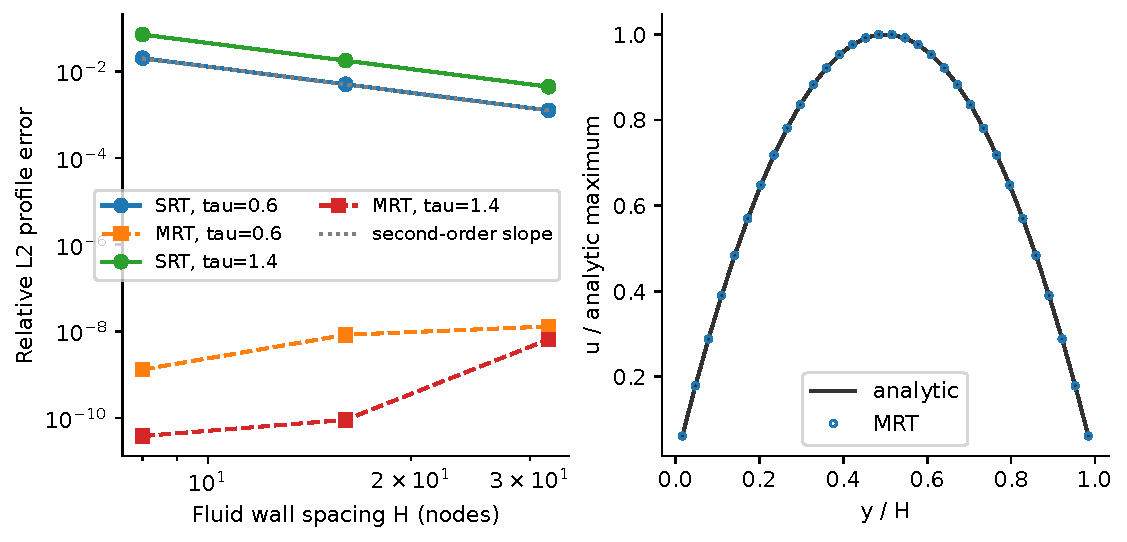
\includegraphics[width=.94\linewidth]{channel-verification.pdf}
\caption{Analytic halfway-wall channel verification. SRT refinement and MRT
profiles are measured independently from globally reconstructed VTI output.}
\label{fig:channel}\end{figure}

Continuous and restarted uniform-force and three-dimensional droplet runs
have bitwise-identical macroscopic fields in six comparisons, including
one-to-two-rank restart. Invalid parameter cases exit with failure. Algebraic
checks of the emitted production coefficients have maximum absolute error
below $9\times10^{-16}$.

For two equal-density layers at viscosity ratio 9:1, the arithmetic
interpolation has 5.37\% relative profile error at $H=64$ against the
sharp-interface solution. Its error against a continuum solution using the
measured diffuse viscosity profile is 0.22\%. Harmonic interpolation reduces
the sharp-interface discrepancy to 0.81\%, while the diffuse-reference error
is 0.23\% (Fig.~\ref{fig:layered}). Thus the major change is a constitutive
transition bias, not an improved collision formula.

\begin{figure}[htbp]\centering
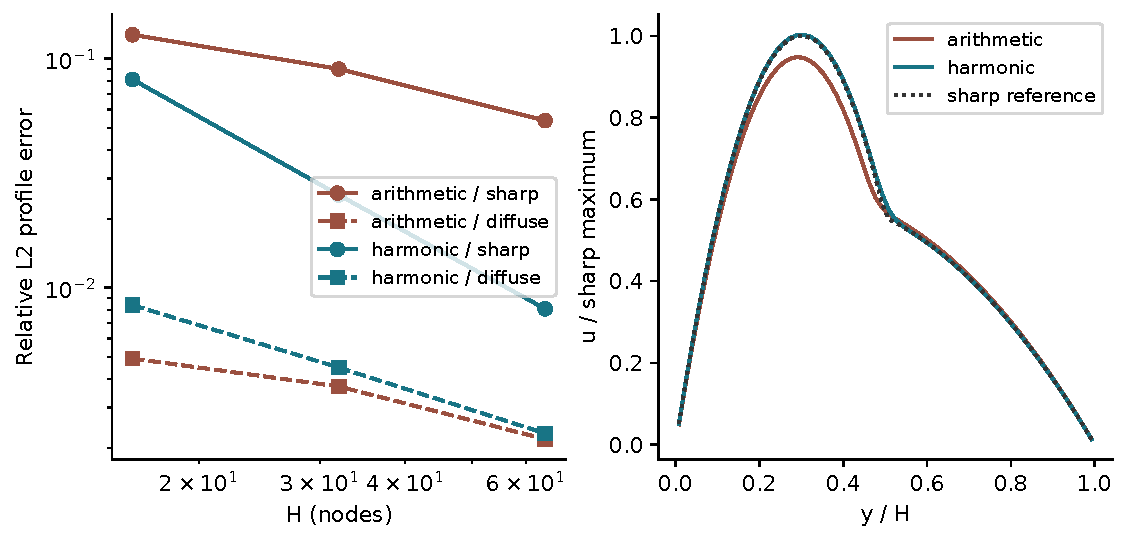
\includegraphics[width=.94\linewidth]{layered-flow.pdf}
\caption{Layered Poiseuille flow: sharp-interface and measured diffuse-profile
references separate viscosity-interpolation bias from discretization error.}
\label{fig:layered}\end{figure}

\subsection{Interfaces and wetting}
Planar interfaces conserve component mass and have spurious speed below
$5\times10^{-16}$. The measured distance between $\chi=-0.9$ and $+0.9$ is
4.765 nodes for D2Q9 and 5.289 for D3Q19 at $\beta=0.7$; D2Q9 widths at
$\beta=0.35$ and 0.9 are 9.376 and 3.929 nodes respectively. Interface width
is measured rather than equated to the input parameter.

Pressure is averaged in bulk regions outside the diffuse interface, and
radius is obtained by orthogonal fitting of subgrid contour intersections.
At 12000 steps, D2Q9 Laplace errors for initial radii 12, 20 and 28 are
1.50\%, 0.50\% and 0.23\%. The D3Q19 errors for radii 8, 12 and 16 are
4.96\%, 1.92\% and 0.99\%; the largest case is continued to 8000 steps.
The smallest spheres contain few interface widths and quantify finite-width
bias, rather than establish a sharp-interface asymptotic regime
(Fig.~\ref{fig:laplace}). Unequal-relaxation cases also retain the prescribed
surface-tension scale; their detailed errors are tabulated in the supplement.

\begin{figure}[htbp]\centering
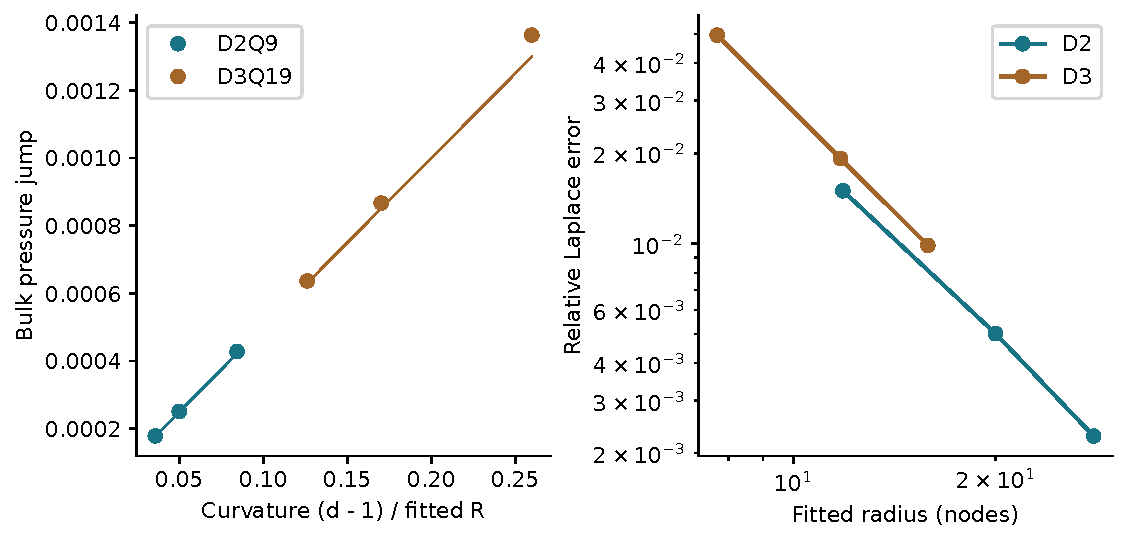
\includegraphics[width=.94\linewidth]{laplace-verification.pdf}
\caption{Laplace pressure compared with $\sigma/R$ and $2\sigma/R$.
Insets quantify finite-interface error; late-time drift is checked separately.}
\label{fig:laplace}\end{figure}

Sessile-drop measurements use the physical halfway wall $y=0.5$ and measure
the angle through phase 1. A principal orthogonal circle fit excludes points
within $0.75W_{0.9}$ of the wall. Sensitivities to contour level and exclusion
height, left--right asymmetry and late-time changes are retained.
For initial radius 36 and $\beta=0.7$, the equilibrated 60-degree measurements
are 64.52 degrees for the clipped stencil and 60.91 degrees for
renormalization. The corresponding 120-degree measurements are 117.18 and
120.92 degrees. Neutral-angle bias persists, and renormalization increases
its spurious speed from approximately $2.8\times10^{-5}$ to $1.05\times10^{-4}$.
This is a tradeoff rather than uniform superiority (Fig.~\ref{fig:wetting}).

\begin{figure}[htbp]\centering
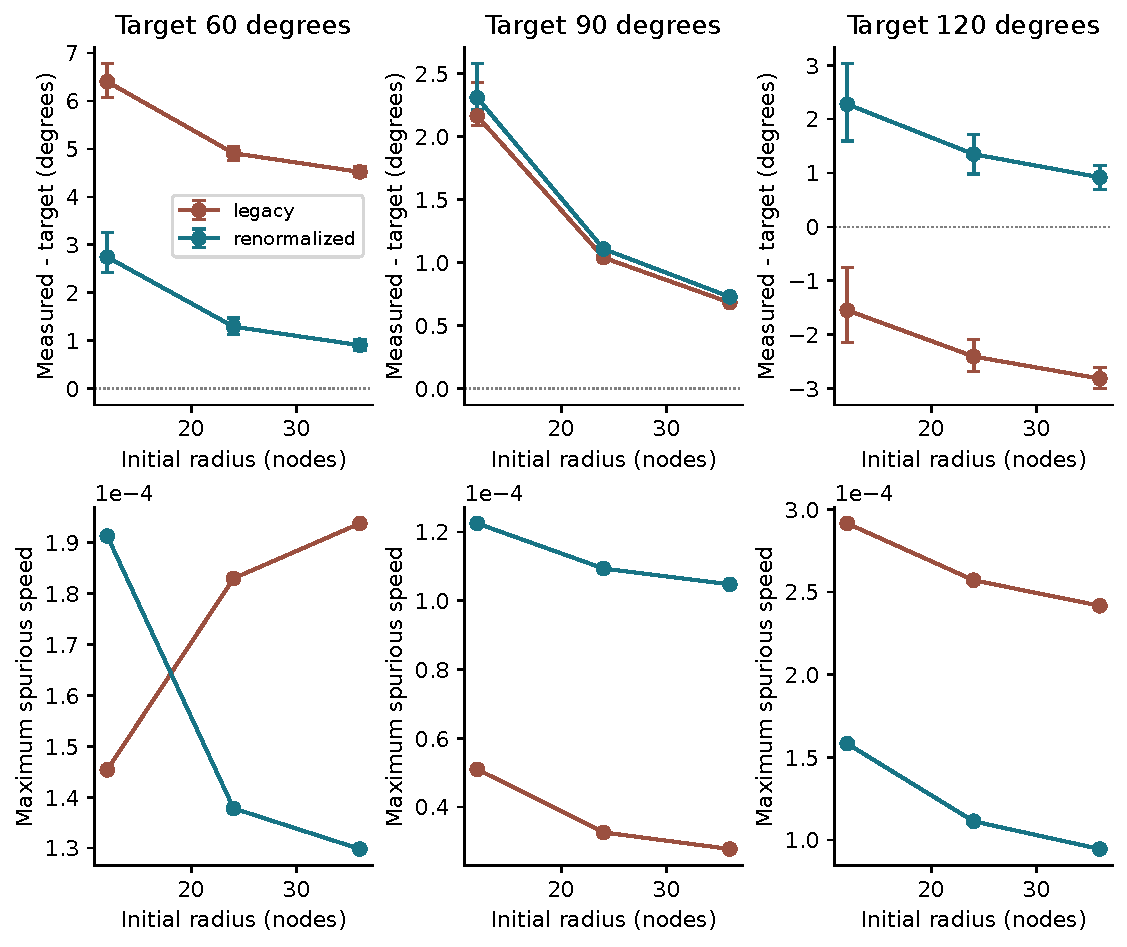
\includegraphics[width=.94\linewidth]{wetting-sensitivity.pdf}
\caption{Flat-wall contact-angle and spurious-velocity ablation. Error envelopes
show deterministic measurement sensitivity rather than statistical confidence.
Size and interface-width sequences use fixed lattice surface tension and are
not labelled a matched-physics spatial convergence study.}
\label{fig:wetting}\end{figure}

\section{Impact and limitations}
The package enables users to reproduce numerical contracts before extending
the solver or porting kernels. It makes source provenance, executable
identity, termination and restart stage inspectable, and provides both
positive results and counterexamples. Prospective applications include
controlled voxel-flow studies and implementation research; current external
adoption or cluster performance is not inferred from source history.

The validation covers equal density, standard pressure weights and the
reported viscosity range. Higher density contrast, moving contact lines,
curved three-dimensional walls, material-junction pinning and thermodynamic
consistency remain unvalidated. Enhanced equilibria and central-moment
developments address wider-density and Galilean-invariance issues
\cite{lafarge2021,saito2023}. Those results cannot be transferred to this
recovered equilibrium without additional changes and tests. Pressure-derived
legacy permeability diagnostics use a reference viscosity and are not used
as validated phase-specific permeabilities in this study. Restart histories
reset conservatively and the native population format is not claimed to be
portable across unlike machine representations.

\section{Conclusions}
DRLab's corrected, inspectable implementation recovers analytic force and
viscosity behavior, conserves component mass in closed domains and supports
consistent restart. Laplace and layered-flow tests bound the multiphase
claims. Wall-stencil renormalization has a clear linear-field rationale and
measurable contact-angle benefits, but also exposes unresolved spurious-flow
and wall-location effects. The verification evidence supports a research
software manuscript within this bounded scope; a claim of a new multiphase
model or universal wetting method is not supported.

\clearpage
\section*{Declarations --- author confirmation required}
\textbf{Software and data availability:} the MIT-licensed implementation,
reproduction scripts and measurement summaries are prepared in
\url{https://github.com/zhou1800/lbflow}. Public access and an immutable release
identifier will be verified before submission.
\textbf{Funding and competing interests:} not yet supplied by the author.
\textbf{AI assistance:} OpenAI Codex and ChatGPT assisted source inspection,
implementation, literature triage and drafting. Numerical claims are tied to
recorded executions or explicit derivations. This disclosure and all final
content require author review before submission.

\bibliographystyle{elsarticle-num}
\bibliography{references}
\end{document}
